\chapter{Basic operations} \label{chap:basicop}

    %\vspace{-1cm}
    \section{Introduction} 
    %\vspace{-0.7cm}
This chapter introduces some of the most basic ingredients of computer programming 
using its foundational concepts of mathematics.
Data types, operators, data structures, etc.
find their origins in mathematical objects.
In a given branch of mathematics, an object is anything that can be formally defined and 
which is subject of deductive reasoning. 
For example, the numbers are objects in the Numbers Theory and
all algebraic structures are objects in Abstract Algebra.
But first let's give some context. 

\textbf{Scientific computing} is considered the third pillar of science. 
Together with a theoretical approach and an experimental approach, 
the complex problems of science and engineering can also be solved 
by means of computers. 
To do that, a computer program is coded following a particular life cycle (see figure \ref{fig:LifeCycle}).
First of all the phenomena of interest must be revised and the \textbf{specifications of the project} defined. 
Then, a \textbf{mathematical model} is built by setting the governing and constitutive equations, the assumptions and constraints of the model, initial and boundary conditions, etc.
With all the tools encompassed in the field of Numerical Analysis, the methods needed to solve the mathematical model are developed, leading to the algorithms. 

An \textbf{algorithm} in mathematics is a finite and ordered sequence of unambiguous instructions to solve a specific problem. 
Notice that this definition involves that i) the algorithm ends in a finite number of steps, 
ii) the sequence of instructions that yields the output are followed in their numerical order and
iii) inputs, instructions and outputs must be properly identified. 

The \textbf{problem} to solve can be seen as a function between a bunch of inputs and their associated outputs.
The algorithm solves an instance of this function, which means, its particularization on a specific set of inputs.
Given a problem, an algorithm to solve it and a machine, 
the theory of computation gives the basis for the automatic processing of the algorithm
and answers things like how efficiently the problem is solved. 

To use machines we need to speak their language, however, machine languages are extremely tough to comprehend by humans.
These languages are known as low-level programming languages and are made of binary numbers carrying processor instructions. 
As an intermediate step, humans use high-level programming languages.
The \textbf{programming code} is the translation or implementation of the algorithm (mathematical language) 
to a language partially understood by the machine, the programming language. 
Notice that an algorithm breaks down a complex problem into simpler instructions 
and then it is translated into a program. 

This program is then compiled or interpreted by a computer program called compiler. 
It is in charge of the final translation from the human-friendly programming language 
into the machine language. As a result, an \textbf{executable code} is generated.
The execution of this code in the machine performs the simulation until the \textbf{numerical results} are obtained.
Here a \textbf{validation} process begins where the output is compared with observations, theoretical models, experiments, etc. 
and the different steps of the cycle are called into question.



 
\usetikzlibrary{shapes.geometric, arrows}

\usetikzlibrary{positioning} 

\tikzstyle{block} = [draw, rectangle, rounded corners, draw=black, very thick,
fill={rgb:orange,1;yellow,2;pink,5},
text width=4cm, text centered, minimum height=1.2cm, node distance=3cm]
\tikzstyle{container} = [draw, rectangle, inner sep=0.3cm]

\tikzstyle{text} = [draw, color=blue]
\tikzstyle{arrow} = [thick,->, >=latex]
\tikzstyle{line} = [thick,-]
 
\begin{figure}[]
\centering

    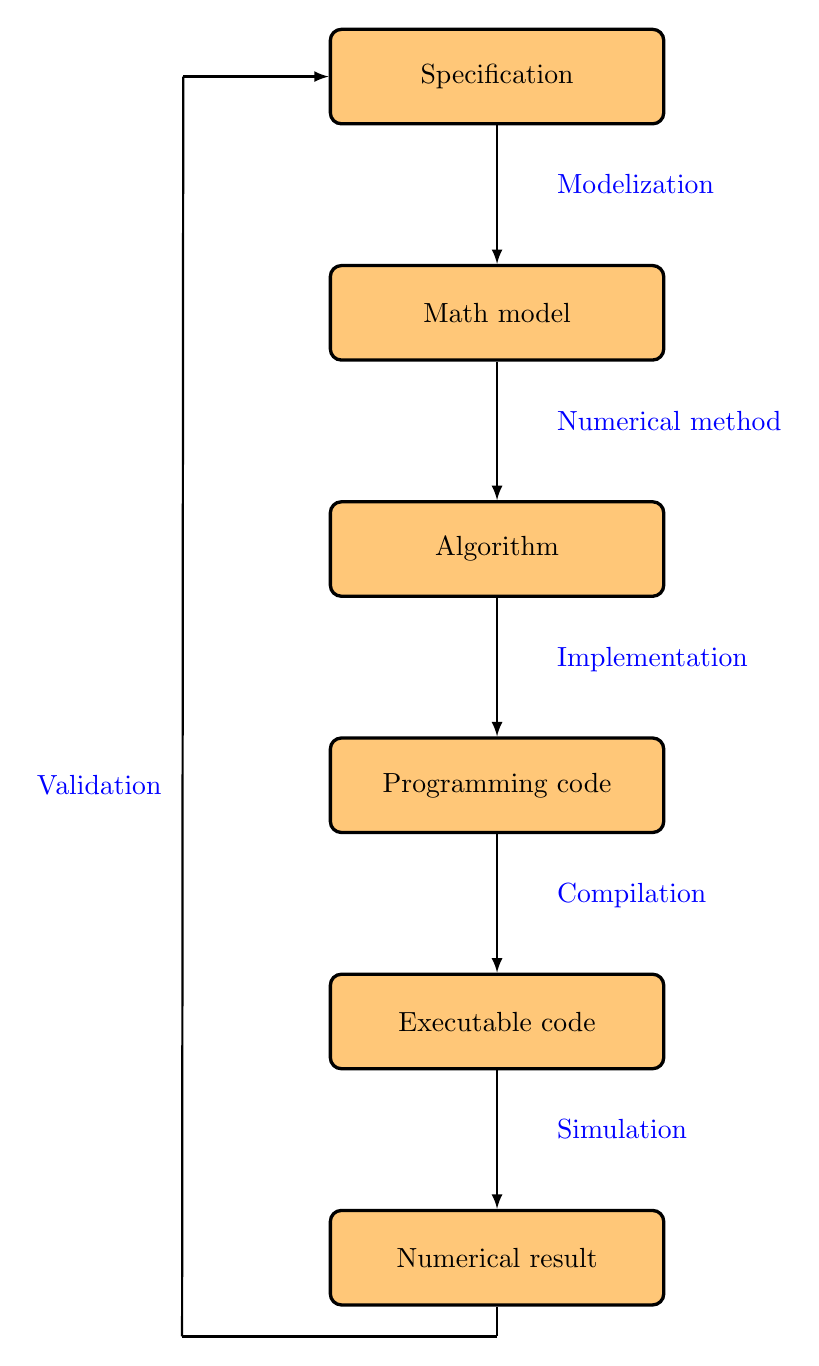
\begin{tikzpicture}
        
        \node [block, name=s] {Specification};
        \node [block, below of=s] (m) {Math model} ;
        \node [block, below of=m] (a) {Algorithm};
        \node [block, below of=a] (p) {Programming code};
        \node [block, below of=p] (e) {Executable code};
        \node [block, below of=e] (r) {Numerical result};
        
        \node [coordinate, below of=r] (d1) {};
        \node [coordinate, left=3cm and 4cm of d1] (d2) {};
        \node [coordinate, left=1cm and 1.847cm of s] (d3) {};
        
        
        \draw [arrow] (s) -- (m);
        \draw [arrow] (m) -- (a);
        \draw [arrow] (a) -- (p);
        \draw [arrow] (p) -- (e);
        \draw [arrow] (e) -- (r);
        
        \draw [line] (r) -- (d1);
        \draw [line] (d1) -- (d2);
        \draw [line] (d2) -- (d3);
        \draw [arrow] (d3) -- (s);
        
        \node [color=blue, left=1cm and 2cm of p] (v) {Validation};
        %  \node [coordinate=0cm and 1cm of s] (m) {Model};
        
        \node [color=blue, below right=0.5cm and -1.5cm of s ]  {Modelization};
        \node [color=blue, below right=0.5cm and -1.5cm of m ]  {Numerical method};
        \node [color=blue, below right=0.5cm and -1.5cm of a ]  {Implementation};
        \node [color=blue, below right=0.5cm and -1.5cm of p ]  {Compilation};
        \node [color=blue, below right=0.5cm and -1.5cm of e ]  {Simulation};
        
        
    \end{tikzpicture}

\caption{Software Development Life Cycle }
\label{fig:LifeCycle}
\end{figure}
 
 
 
 
 
 
 
 
 
 
 
 
 
 
 
 
 \newpage
Most high-level programming languages use the same components as building blocks to translate the algorithm instructions:
\begin{itemize}[noitemsep]
    \item \textbf{Statements and Expressions:} Statements are all line of code that instructs the compiler to perform a task.
    There are several types of statements like assignments, procedures calls, input/output statements or control flow structures. 
    It is usually distinguished between statement and expression. 
    The former is executed with no value as a result, only a compiler instruction, 
    the latter is evaluated and ends with a resulting value.
    \begin{itemize}
        \item \textbf{Control flow structures:} These are the structures that, by means of keywords, allow to control the flow of data along the program. 
        The most basic control structures are the loops, which let instructions be repeated until a condition is reached and 
        the conditionals, which allow to make decisions and execute instructions accordingly.  
    \end{itemize}
    
    \item \textbf{Variables and Data structures:} A variable involves a tag that identifies a memory location and 
    the content of the memory, the data itself. 
    This attached data, of different types (integer, real, character, etc.), may change during the execution of the program.
    In contrast, \textbf{constants} may also have a name but the data don't change during the execution.
    Data structures are also used to store, organize and process data, 
    now arranged in a specific way so that it can be treated efficiently. 
    Some common data structures are arrays, sets, lists, tuples, trees, graphs, etc.
    
    \item \textbf{Operators:} Symbols that tell the compiler to perform operations of different kind in order to produce a result.
    There are arithmetic operators ($+$, $*$, $-$, $/$, etc.), 
    relational ($>$, $<$, $==$, etc.), 
    logical operators (\texttt{AND}, \texttt{OR}, \texttt{NOT}), etc. 
    Sometimes the assignment operator (\texttt{=}) is also included in this classification, 
    however, it has a different nature. 
    
    \item \textbf{Functions, Procedures:} Procedures and functions in computer science are usually defined as 
    named blocks of code that are called to perform a task, maybe accepting some input arguments and maybe returning some output values. 
    Pure functions can be included here, the representation of the mathematical functions in programming. 
    
    \item \textbf{Objects:} objects are constructions with 
    \textit{state} (combinations of variables and data structures) and 
    \textit{behaviour} (combinations of functions and methods) 
    to represent concepts and objects of the real world. 
    A complex number could be an object, 
    whose state needs from variables: the real and imaginary parts, and 
    whose behaviour involves addition, multiplication, conjugation among others. 
    
    \item \textbf{Comments:} Lines of code intended to help programmers understand the code, 
    but which are not read or executed by the compiler.
\end{itemize}
\vspace{-0.5cm}
Other \textbf{keywords and characters} are usually reserved by each programming language 
in order to perform tasks like: 
group expressions (parenthesis), 
delimit characters (\texttt{''}), 
break lines of code, 
include more than one statement in a line, etc.

Finally, the \textbf{compiler/interpreter directives} are not part of the programming language itself 
but also instructs the compiler to perform tasks. 
These statements cause the compiler to take a specific action during compilation and 
may vary from compiler to compiler.
 
 
Let's see all these components together, 
do not worry if the syntax of the languages or 
the meaning of the keywords are not clear at this point. 
The first example solves the roots of a second degree equation in Fortran and 
the other example reads real and imaginary parts of a complex number with Python.


\begin{figure}[h]
    \centering
    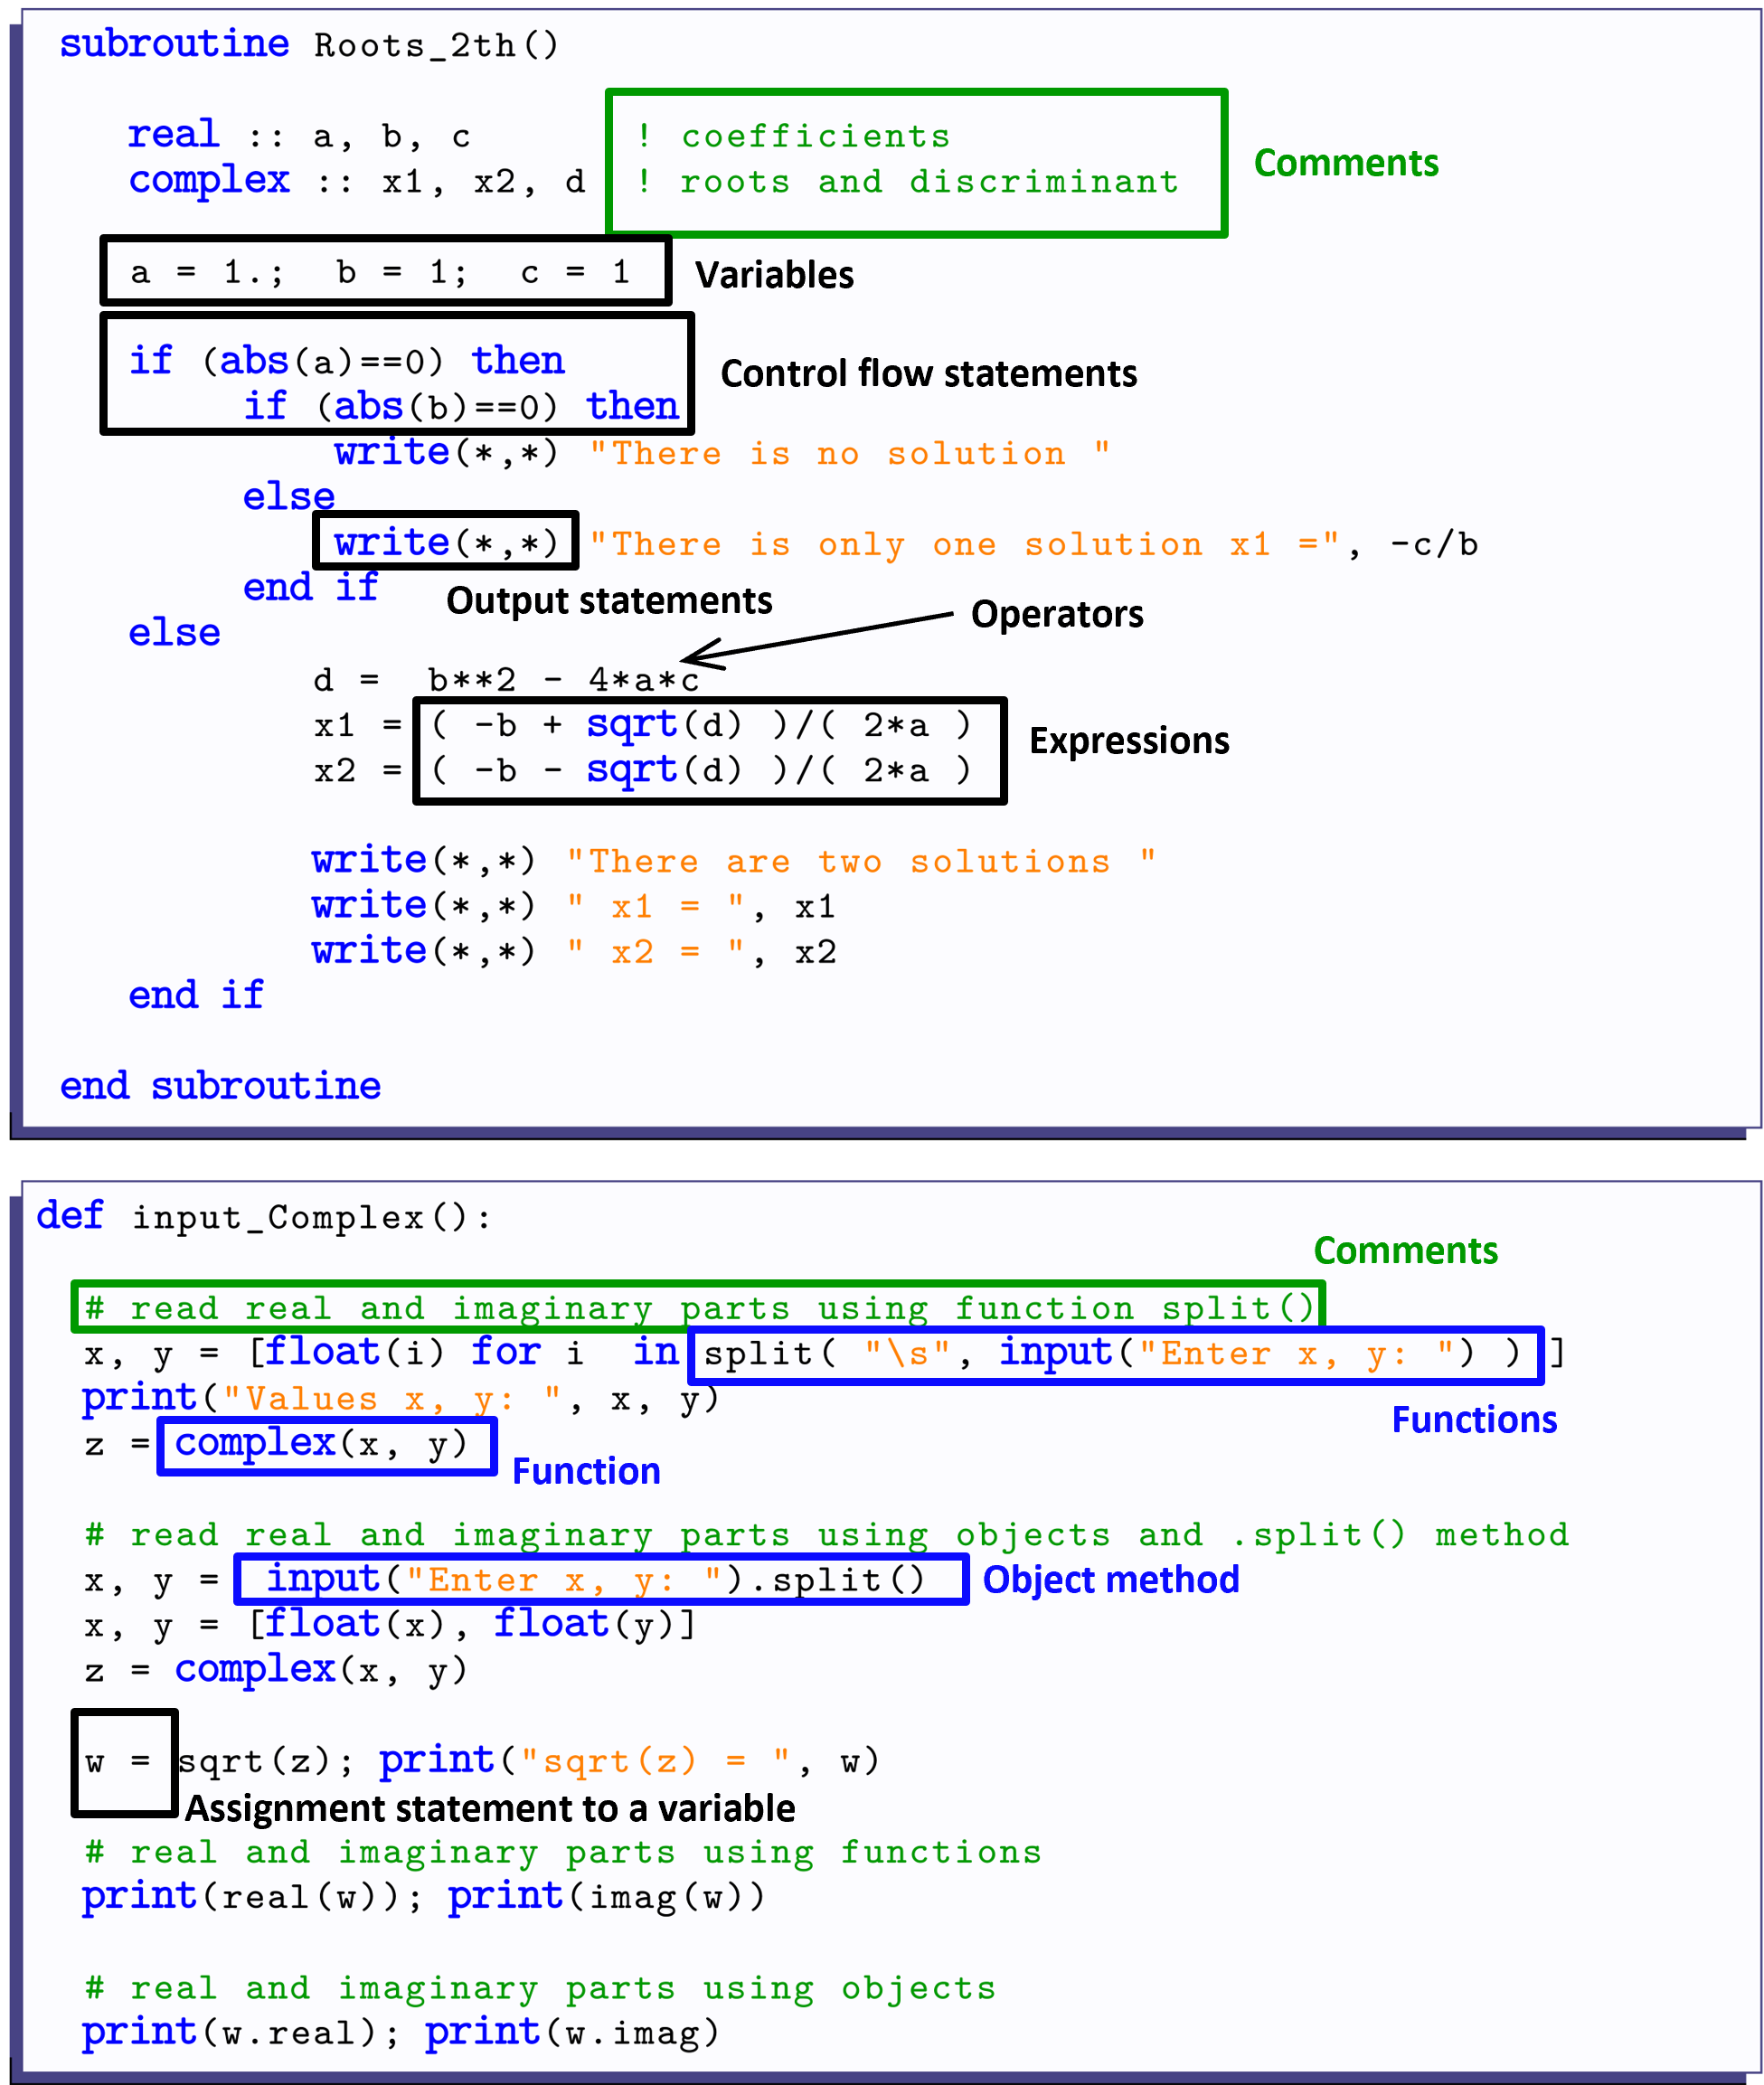
\includegraphics[width=.95\textwidth]{./doc/Figures/components.png}
    \caption{Main building blocks used to code in common programming languages.}
    \label{fig:components}
\end{figure}
\FloatBarrier
 %THIS CODE IS USED TO GENERATE LATER THE IMAGE...
 %\vspace{0.5cm}
 %\renewcommand{\home}{./Fortran/sources/Foundations/Roots} 
 %\lstfor
 %\listings{\home/Roots.f90}{subroutine Roots_2th}{end subroutine}{}
 %
 %\renewcommand{\home}{./Python/sources/Foundations/Data_type} 
 %\lstpython
 %\listingsp{\home/data_type.py}{def input_Complex}{w.imag}{}










%MORE:
%Input: getting data and commands into the computer
%Output: getting your results out of the computer

%Libro FORTRAN: Programación Multicapa

%Most important basic elements for programming languages are:
%Programming Environment
%Keywords
%Input and Output Operations

%Functions
%A function is a statement that returns a value. For example, the function InputBox() returns the value of its dialog text field.
%Objects
%An object is a program “building block” entity. It can be visible, like a Button control, or invisible like a Timer control.
%Properties
%A property is a characteristic of an object. For example, the property Btn.Text is the Text property of the Btn object.
%Methods
%A method is an action that an object can perform. For example, the method Btn.Click() is the Click method of the Btn object.



%The assignment statement \texttt{v = 3*5 + 2} becomes the bottleneck of programming languages in the sense that a program is mainly concerned 
%with the flow of assignments of single variables (imitating single words). 
%By executing assignments many times, maybe altering subscripts (imitating memory addresses), 
%the program ends up with the result stored in a variable (imitating the storage in memory). 
%Furthermore, this assignment statement splits the programming languages into two worlds: 
%a world of expressions with strong algebraic properties (\texttt{3*5 + 2}) and a world of statements with few mathematical properties (\texttt{v =}).



    \section{Data types and their operators}
    
Several objects are used to build the different branches of mathematics; numbers, operations, functions, sets, vectors, matrices, tensors and a large etcetera. 
Let's review here the formal definition of some objects that later are represented in programming by means of the data types. 

In mathematics, the numbers are usually classified into sets according to their nature.
The set of \textbf{integers} $\mathbb{Z}$ includes the number zero (0), the natural numbers ($\mathbb{N} = \{ 1,2,3,... \}$) and their additive inverses ($\{ -1,-2,-3,... \}$), the negative numbers.
The set of \textbf{real} numbers ($\mathbb{R}$) includes any number identified with a point on the real number line.
$\mathbb{R}$ includes both the set of rational numbers ($\mathbb{Q}$) and the set of irrational numbers.
Finally, the \textbf{complex} numbers ($\mathbb{C}$) extends the real numbers using the imaginary unit, an element satisfying the equation $i^2 = -1$, which does not have solution among the reals.
Once introduced the imaginary unit, every complex number can be expressed as $a+bi$ where $a,b\in\mathbb{R}$. 

The fact that a number belongs to one or another set is not only important from the classification point of view.
It also comes with a long list of derived consequences which are essential to build mathematics. 
Let's take for example $\mathbb{Z}$ equipped with the usual \textbf{arithmetic operations} of addition and multiplication and the usual ordering. 
Automatically we can assert that for any $a,b\in\mathbb{Z}$, $a\cdot b\in\mathbb{Z}$ and $a+b\in\mathbb{Z}$.
Also, we do not have to worry about the order to operate them since $a+b=b+a$ and $a\cdot b = b\cdot a$.
To mention other results, for $a,b>0$ then $a+b>0$, $a+b>a$, $a+b>b$, $a\cdot b>0$, $a\cdot b\geq a$, $a\cdot b\geq b$, the equation $a+x = 0$ has a unique solution $x\in\mathbb{Z}$, etc.

From the axioms some properties emerge and other properties are built on these until a whole theory around the integers is built.
The same happens with $\mathbb{N}$, $\mathbb{R}$, $\mathbb{C}$, etc. 
When we use these mathematical objects in a computer, 
it's not only the elements of the set but also
all the properties and results derived. 

However, the arithmetic operators are not the only essential operators in mathematics, 
in the context of ordered sets like $\{\mathbb{R}\}$ or $\{\mathbb{Z}\}$,
any two elements can be compared with the usual ordering, 
which is derived from the 
conventional counting and measuring order on $\mathbb{R}$. 
The \textbf{relational operators} are used to compare any two numbers. 
Both numbers could accomplish with some of the following comparisons: 
equals operator $x = y$, not equal $x\neq y$, less than $x < y$, greater than $x > y$, less or equal than $x \leq y$ and greater or equal than $x\geq y$. 
Notice that the complex numbers do not have the structure of an ordered field and then, these operators are not useful in this context. 


\newpage
Jumping to the context of Boolean algebra, the same principle applies.
However, now the elements to consider are the truth values: \textit{true} and \textit{false}, instead of numbers.
In addition, the basic operations between these elements are conjunction (and), disjunction (or) and negation (not) 
instead of binary operations like addition and multiplication.
These operations allow to combine one or more mathematical statements to create a new one 
and are usually represented by the \textbf{logical operators}.
Given the statements $P$ and $Q$:
\begin{enumerate}[noitemsep]
    \item Conjunction of statements: $P \land Q$ is true when both $P$ and $Q$ are true.
    \item Disjunction of statements: $P\lor Q$ is true when at least $P$ or $Q$ is true.
    \item Negation of a statement: $\neg P$ is true only when $P$ is false.
    \item Implication or conditional: If $P$ then $Q$, $P\to Q$ is false only when $P$ is true and $Q$ is false. 
    \item Equivalent: $P = Q$ or $P \iff Q$ is true if both functional arguments have the same logical value
    \item Non-equivalent: $P \neq Q$ is true if both functional arguments have different logical value
\end{enumerate}
%More than one operator can be used together in an statement building a compound operator.


 

%PROGRAMMING
As a need of representing these essential mathematical sets in the computer, data types are used. 
Each constant, variable, array or function in a language has an intrinsic data type associated, a set to which they belong. 
In the same way, the mentioned \textbf{arithmetic, comparison and boolean operations} are reproduced in the programming language 
so the whole potential of the algebraic structures are transmitted to the computer. 
Hence, the data type decides, among other things, the allowed values that the entity can have and the set of operations that can be performed with them.

Roughly speaking, a value $n\in \mathbb{Z}$ is stored in an \texttt{integer}, 
$x\in \mathbb{R}$ is stored in a \texttt{real} and 
$z\in \mathbb{C}$ is stored in a \texttt{complex} variable.
Many nuances to the equivalence between the programming concept and the mathematical abstraction 
for integers and reals are treated in the Part \ref{PartII} of this book. 

The \texttt{logical} type gets the two possible values of the Boolean algebra; \texttt{True} and \texttt{False}. 
Finally, the \texttt{character} type can store strings with ASCII (American Standard Code for Information Interchange) characters which includes alphanumeric, symbols and sign characters.

Programming languages usually have built-in all the needed operations through \textit{operators} in their syntax,
hence, each of them has a reserved symbol or keyword.
From a general perspective, 
they behave similarly to functions (also treated in this book), 
but they differ in the syntax or the semantics. 
Furthermore, sometimes the language allows the users to create new operators 
or add meanings to existing ones similarly to functions. 





        \newpage
        \subsection*{Fortran code}
        \vspace{-.5cm}
Fortran provides five intrinsic data types:
\begin{itemize}[noitemsep]
    \item Numeric nature: \texttt{integer}, \texttt{real}, \texttt{complex}. 
    \item Boolean nature: \texttt{logical}.
    \item Text nature: \texttt{character}.
\end{itemize}
Fortran has a \textbf{explicit} data typing, which means that before using any variable, all must be previously declared with a specific type.
The code below shows the declaration and initialization of the five intrinsic data types: 
\vspace{0.5cm}
\lstfor
\renewcommand{\home}{./Fortran/sources/Foundations/Basic operations} 
\listings{\home/Basic_operations.f90}{subroutine Data_types}
{end subroutine}{Basic_operations.f90}

\begin{table}[!h]
    \centering
    \begin{tabular}{|l|l|l|l|}
        \hline
        Data Type  & Operator type & Operator & Meaning \\ \hline
        Numeric & Arithmetic & + & Addition \\ 
        ~ & ~ & \texttt{-} & Subtraction \\ 
        ~ & ~ & \texttt{*} & Multiplication \\ 
        ~ & ~ & \texttt{/} & Division (integers!) \\ 
        ~ & ~ & \texttt{**} & Exponentiation \\ 
        ~ & Relational & \texttt{==}   & Equal to (\texttt{=} not valid!) \\ 
        ~ & ~ & \texttt{/=}   & Not equal to \\ 
        ~ & {\footnotesize (no \texttt{complex})} & \texttt{>}   & Greater than  \\ 
        ~ & {\footnotesize (no \texttt{complex})} & \texttt{<}  & Less than \\ 
        ~ & {\footnotesize (no \texttt{complex})} & \texttt{>=} & Greater or equal to \\ 
        ~ & {\footnotesize (no \texttt{complex})} & \texttt{<=}   & Less or equal to  \\ \hline
        \texttt{logical} & Logical & \texttt{.and.} & Conjunction \\ 
        ~ & ~ & \texttt{.or.} & Disjunction \\ 
        ~ & ~ & \texttt{.not.} & Negation \\ 
        ~ & Relational &\texttt{==}  & Equivalent \\ 
        ~ & ~ & \texttt{/=}   & Not equivalent \\ \hline
        \texttt{character} & Character & \texttt{//} & Concatenate \\ 
        ~ & Relational & \texttt{==,/=,>,>=,<,<=} & order ASCII table \\ \hline
    \end{tabular}
\end{table}

%We don't tell the options .EQ., .NEQ., etc.
%Neither the .eqv. and .neqv. in logical



        \newpage 
        \subsection*{Python code}
        \vspace{-.5cm}
The same five data types (also known as primitive data types) are built-in in Python:
\vspace{-0.2cm}
\begin{itemize}[noitemsep]
    \item Numeric nature: \texttt{int}, \texttt{float}, \texttt{complex}. 
    \item Boolean nature: \texttt{bool}.
    \item Text nature: \texttt{str}.
\end{itemize}
\vspace{-0.2cm}
Since Python is mainly an implicit typing language we don't declare the type of any variable and just initialize it.
The following program shows an example of the initialization of the five data types we can find: 
%\vspace{0.5cm} 
\renewcommand{\home}{./Python/sources/Foundations/Data_type} 
\lstpython
\listingsp{\home/data_type.py}{def data_types}
{string}{data_type.py}

\begin{table}[!h]
    \centering
    \begin{tabular}{|l|l|l|l|}
        \hline
        Data Type  & Operator type & Operator & Meaning \\ \hline
        Numeric & Arithmetic & + & Addition \\ 
        ~ & ~ & \texttt{-} & Subtraction \\ 
        ~ & ~ & \texttt{*} & Multiplication \\ 
        ~ & ~ & \texttt{/} & Division \\ 
        ~ & ~ & \texttt{**} & Exponentiation \\ 
        ~ & ~ & \texttt{\%} & Modulus \\
        ~ & ~ & \texttt{//} & Floor division \\
        ~ & Relational & \texttt{==}   & Equal to (\texttt{=} not valid!) \\ 
        ~ & ~ & \texttt{!=}  & Not equal to \\ 
        ~ & {\footnotesize (no \texttt{complex})} & \texttt{>}  & Greater than  \\ 
        ~ & {\footnotesize (no \texttt{complex})} & \texttt{<}  & Less than \\ 
        ~ & {\footnotesize (no \texttt{complex})} & \texttt{>=}  & Greater or equal to \\ 
        ~ & {\footnotesize (no \texttt{complex})} & \texttt{<=}   & Less or equal to  \\ \hline
        \texttt{bool} & Logical & \texttt{and} & Conjunction \\ 
        ~ & ~ & \texttt{or} & Disjunction \\ 
        ~ & ~ & \texttt{not} & Negation \\  
        ~ & Relational &\texttt{==} & Equivalent \\ 
        ~ & ~ & \texttt{!=}  & Not equivalent \\ \hline
        \texttt{str} & Character & \texttt{+} & Concatenate \\ 
        ~ & {\footnotesize needs \texttt{int}} & \texttt{*} & Repetition \\ 
        ~ & ~ & \texttt{in} & Membership \\
        ~ & ~ & \texttt{not in} & Not membership \\
        ~ & Relational & \texttt{==,/=,>,>=,<,<=} & order ASCII table \\ \hline
    \end{tabular}
\end{table}


%Furthermore, while some programming languages allow the use of some data types as if they were a different type (weak typing) others does not (strong typing). 

        \subsection*{Operators}

The operators presented in the tables above are now coded into some examples. 
In the first example we consider a well known equality, the Euler's identity:
$$
e^{i\pi}+1 = 0
$$
In the second one we consider a simple inequality and check the fact that inequalities 
must reverse their sign when both sides are multiplied or divided by a negative value. 
For a given $x,y\in\mathbb{R}$ with $x\leq y$ it is clear that:
$$
-x \geq -y
$$
In the third example the string \texttt{abcdef} is compared alphabetically with \texttt{abcdeg}. 

\vspace{0.5cm}
\lstfor
\renewcommand{\home}{./Fortran/sources/Foundations/Basic operations} 
\listings{\home/Basic_operations.f90}{subroutine Operators}
{end subroutine}{Basic_operations.f90}

\vspace{0.5cm} 
\lstpython
\renewcommand{\home}{./Python/sources/Foundations/data_type} 
\listingsp{\home/data_type.py}{def Operators}{abc}{data_type.py}







    \newpage
    \section{Assignment operator}
The assignment operator is different from the rest of operators in the sense that its 
definition does not come from pure mathematics, it is not related to the mathematical equality 
but related to the assignment statement. 
We have seen that the variables are built by 
a memory storage location tagged with a symbolic name.
While the name is just a tag to identify the data,
the content of the memory location (value) is the data itself. 
Essentially, this operator sets or re-sets the value stored in that memory location (data) using its name. 

To do that the assignment statement is used: 

\texttt{name = expression}

This statement works from right to left, first the \texttt{expression} on the right is evaluated and
when it is done, the data resulted is charged in the memory location tagged by \texttt{name}.
Actually, for some programming languages it is referenced as the left arrow $\leftarrow$ indicating its purpose.
According to John Backus in his article ``Can Programming Be Liberated from the von Neumann Style?'' 
this operator splits the programming languages into two worlds: 
a world of expressions with strong algebraic properties \texttt{expression} and 
a world of statements with few mathematical properties \texttt{name =}.
\vspace{0.5cm}
\lstfor
\listings{./doc/Figures/assignment.f90}{x}{12}{assignment.f90}

%Several variations of the assignment operator are sometimes defined in languages like Python. 
%For example, 
%an operator that adds the right side operand with the left side and then assign the result to the left operand: \texttt{+=}.
%Also, an operator that multiplies the right operand with the left operand and then assign the result to left operand: \texttt{*=}.
%Like this, the following options are allowed: \texttt{-=}, \texttt{/=}, \texttt{\%=}, \texttt{\^{}=}, \texttt{//=}, \texttt{**=}, \texttt{\&=}, \texttt{|=}, \texttt{>>=}, \texttt{<<=}. 






    \newpage
    \section{Control Flow statements}
In order to translate the steps of an algorithm to the programming language 
and essentially manage the flow of data, the control flow statements are needed. 
All the statements in a program are executed from top to bottom but 
the control flow statements modify this behaviour by including decisions, 
loops, branches, separate block executions, etc.
Let's review some essential statements commonly used, 
specially in imperative programming languages 
(we will delve into the concepts of imperative and declarative languages later in this book).


        \subsection{Conditionals}
        \vspace{-0.3cm}
The conditionals are used to separate the flow into branches depending on logical conditions. 
Some statements are executed if a logical expression is evaluated as \texttt{true} and others if it is evaluated as \texttt{false}.

An \texttt{if - then - else} structure is used to evaluate first the condition between parenthesis and execute some statements if it's \texttt{true}.
If the condition is evaluated as \texttt{false} then the statements within the \texttt{else} statement are executed. 
Although \texttt{else} is optional, we strongly recommend to include it in every conditional structure to ensure that at least one of the branches is executed. 
If it seems to be not necessary then write just an error message within the \texttt{else} (see examples). 
A conditional is used to code the absolute value of a number in the examples below. 

The structure \texttt{if - elseif - else} works in the same way, however it allows more than two branches in the same structure. 
From top to bottom all the conditions are evaluated, if one condition is \texttt{false} it jumps to check the following one. 
In the moment that one condition is \texttt{true}, their statements are executed and the structure exited without checking the rest. 
If neither condition is met, the \texttt{else} block of code is executed.
As an example let's compare two integers $a$ and $b$. 

Fortran implements a third kind of conditional, the \texttt{case} structure. 
It executes a block of statements depending on the value of an \texttt{integer} or \texttt{character} expression.
All the Fortran menus in this book are coded using this structure. 
Consider for example the menu of Foundations: 
the user introduces an integer which is stored in \texttt{option} and 
\texttt{select case(option)} is executed accordingly. 
If \texttt{option} is \texttt{2}, the statements under \texttt{case(2)} are executed. 

Notice the differences between both languages. 
In Python the indentation rules must be strictly followed, 
the colon symbol is used before starting the body of the conditional and 
the keywords are \texttt{if}, \texttt{elif}, \texttt{else}.
In Fortran, instead of indentation, the \texttt{end} statement indicates where the body of the conditional ends and 
the keywords are \texttt{if}, \texttt{elseif}, \texttt{else}.


            \newpage
            \subsubsection*{Fortran code} 
            %\vspace{0.5cm}
            \lstfor
            \renewcommand{\home}{./Fortran/sources/Foundations/Basic operations} 
            \listings{\home/Basic_operations.f90}{else conditional}
            {end subroutine}{Basic_operations.f90}
        
        
            \subsubsection*{Python code}
            %\vspace{0.5cm} 
            \lstpython
            \renewcommand{\home}{./Python/sources/Foundations/data_type} 
            \listingsp{\home/data_type.py}{else conditional}{Error}{data_type.py}




        \newpage
        \subsection{Loops}

Loops are used to repeat a bunch of statements cyclically, whether it is executed 
a fixed number of times, 
until a condition is reached or 
maybe up to infinity. 
Typically, the statements inside the loop are executed and then some condition is checked.
Depending on this condition (\texttt{true} or \texttt{false}) the bunch of statements starts again from the beginning or
the loop is exited and the next instruction outside the loop is executed. 

Two basic types of loops are usually used depending 
if the number of iterations is explicitly known or 
it is not but a stop condition is known. 
In the first case, an index controls the loop: it usually has start and stop values and sometimes the increment in each iteration is specified.
Notice that this index cannot be modified inside the loop.
In the second case the number of iterations is not determined beforehand but 
the loop finishes once a condition is evaluated as \texttt{false}. 
This conditions is usually determined by some variables modified inside the loop.

However, some keywords positioned inside a loop can be used to transfer 
some control of the loop execution to the statements inside. 
\begin{itemize}
    \item Use \texttt{exit} in Fortran or \texttt{break} in Python to finish its execution and skip to the next code after the loop. 
    Notice that these statements are usually positioned within a conditional so the loop is finished if the condition is \texttt{true}.        
    \item Use \texttt{continue} in Python to end the current iteration of the loop but continue with the following iteration. 
\end{itemize}

In the examples below we first compute the factorial of a number $n$, $n!$.
Since we know the number of multiplications to perform (given by \texttt{n}) we can use a 
\texttt{do} loop in Fortran and 
\texttt{for} loop in Python.
Notice that in both cases the multiplication stops when multiplying by 2, 
while in Fortran this is expressed by the stop value 2 (\texttt{n, 2, -1}) (sequence $(n, n-1, n-2,...,2)$), 
in Python the \texttt{range} function does not take the stop value at any moment in the sequence
so it has to be expressed as \texttt{range( n, 1, -1 )} (sequence $(n, n-1, n-2,..., 2)$).

Later, the Newton-Raphson method is used to find a good approximation for one root of $f(x) = 3x^3-x^2$. 
We do not know the amount of iterations needed to find the root but we can set as condition that 
the distance between two successive approximations, $|x_{n+1} - x_n|$ is less than $0.00001$ so, while this error condition 
is higher than our threshold, the loop continues iterating.

Finally notice the differences between both languages. 
In Python the indentation rules must be strictly followed and the colon symbol is used before starting the body of the loop.
In Fortran, instead of indentation, the \texttt{end} statement indicates where the body of the loop ends. 


            \newpage
            \subsubsection*{Fortran code} 
            \vspace{0.5cm}
            \lstfor
            \renewcommand{\home}{./Fortran/sources/Foundations/Basic operations} 
            \listings{\home/Basic_operations.f90}{Flow_structures}
            {One root of}{Basic_operations.f90}
            
            
            \subsubsection*{Python code}
            \vspace{0.5cm} 
            \lstpython
            \renewcommand{\home}{./Python/sources/Foundations/data_type} 
            \listingsp{\home/data_type.py}{def Flow_structures}{One root of}{data_type.py}



    \newpage 
    \section{Example: Roots of a second degree equation} 
In this section all of the concepts presented above are put into practice, 
a program to obtain the roots of a second order equation is presented:  
$$
a x^2 + b x + c = 0, \qquad \forall \ a, b, c \in \mathbb{R}.
$$
The fundamental theorem of algebra states that every  Nth order polynomial has N complex roots. 
If the coefficients are real, then the roots are complex conjugate.
Dividing the above equation by $ a $ an looking for a perfect square, 
the following equation is obtained: 
$$
\left( x + \frac{b}{2a} \right)^2 - \frac{b^2 }{ 4 a^2} + \frac{c}{a} = 0. 
$$
Solving the unknown $x$, the well known formula for the roots is obtained: 
\begin{equation}
    x_{1,2} = \frac{ - b \pm \sqrt{ b^2 - 4 a c }  }{ 2 a  }  
    \label{x12}
\end{equation} 
If the discriminant $ d = b^2 - 4 a c $ is less than zero, roots become complex. 
In the following code, complex solutions given by (\ref{x12}) are implemented. 
Note that the discriminant $ d $ was defined as a complex variable to avoid maths problems 
when the discriminant is negative. Whereas negative numbers do not have real square roots, 
they have a value within the set of complex numbers. 

\vspace{0.5cm}
\renewcommand{\home}{./Fortran/sources/Foundations/Roots} 
\lstfor
\listings{\home/Roots.f90}{subroutine Roots_2th}{end subroutine}{Roots.f90}


        \newpage 
        \subsection*{Python code}
The same function is presented now coded with Python. Essentially both codes are quite similar, 
however, now data types for variables are not explicitly declared because 
Python automatically declares them. In addition, indentation rules must be strictly followed. 
\vspace{0.5cm} 
\lstpython
\renewcommand{\home}{./Python/sources/Foundations/Roots} 
\listingsp{\home/Roots.py}{from}{output}{Roots.py}








% -----------------------------------  UNTIL   HERE BASICs  -----------------------------------













    \newpage
    \section{Data structures} 
\vspace{-0.5cm}
Numbers and truth values are not the only objects needed to build the different branches of mathematics.
Also sets, vectors, tuples, matrices, tensors or sequences are used in the context of algebra, calculus or set theory.
Let's review now the formal definition of the objects that are represented in programming by arrays, sets, tuples, lists and dictionaries. 

\begin{enumerate}[noitemsep]
    \item \textbf{Set:} gathering together into a whole of definite, distinct objects of our perception or our thought.
    \item \textbf{Tuples and sequences:} enumerated collection of elements, where repetitions are allowed and order matters. 
    While a sequence can be finite or infinite, a tuple is always finite. 
    \item \textbf{Vectors:} elements of a vector space.
    \item \textbf{Matrices:} rectangular arrangement of numbers (or other mathematical objects) distributed in rows and columns.
    \item \textbf{Graphs:} mathematical structures used to model pairwise relations between objects.
    \item \textbf{Array:} an orderly arrangement of similar mathematical objects.
\end{enumerate}

        \subsection*{Set}
\vspace{-0.5cm}
% --------------------------------------------------------------
A \textbf{set}, with the definition given by Georg Cantor within the set theory, 
is a gathering together into a whole of definite, distinct objects of our perception or our thought, 
which are called elements of the set.
The elements of a set can be any mathematical objects: numbers, points in space, geometrical shapes, variables or other sets.
However, every element of the set must be different from the others.
Sets are usually indicated by listing its elements between curly brackets separated by commas (roster notation): $\{\textrm{car, boat, plane}\}$.

Given two sets $A$ and $B$, the following operations can be performed:
\begin{enumerate}[noitemsep]
    \item Union: $A\cup B$ is the set of elements that belong to set $A$, set $B$ or both.
    \item Intersection: $A\cap B$ is the set of elements that belong to set $A$ and $B$.
    \item Difference: $A - B$ is the set of elements that are in $A$ but not in $B$.
    \item Complement: $\overline{A}$ is the set of all elements that are in the universal set $S$ but are not in $A$.
\end{enumerate}
It is interesting to extend the use of propositional logic to the set theory. 
Notice that an element or set do not have a truth value associated, they are not true or false by themselves. 
By including some relational operators, true or false statements can be 
built and used in the context of propositional logic. 
For example, we can say $3.5 \in \mathbb{R}$ which is true. 

\newpage
Given a set $A$, the following operators are used:
\vspace{-.5cm}
\begin{enumerate}[noitemsep]
    \item Membership: $x\in A$ means that $x$ is an element of the set $A$. The opposite operator would be $x\notin A$.
    \item Subset: $A \subseteq B$ means that all elements of $A$ are also elements of $B$.
    \item Superset: $A \supseteq B$ means that all elements of $B$ are also elements of $A$.
    \item Strict subset: $A \subset B$ means that all elements of $A$ are also elements of $B$ but they are not equal.
    \item Strict superset: $A \supset B$ means that all elements of $B$ are also elements of $A$ but they are not equal.
\end{enumerate}
\vspace{-.5cm}

        \vspace{-.5cm}
        \subsection*{Sequence and Tuple}
        \vspace{-.5cm}
% --------------------------------------------------------------
\textbf{Tuples and sequences} are also collections of mathematical objects.
However, a \textbf{sequence} is an enumerated collection, where repetitions are allowed and order matters.
Unlike sets, since the elements follow an order, they can be repeated in different positions of the sequence.
The length of a sequence is its number of elements and could be any finite value or infinite.
A sequence can also be interpreted (and it usually is) as a function whose domain is a countably ordered set like $\mathbb{N}$ 
(denoting the position within the sequence) to the set of elements. 
Sequences are essential in different branches of mathematics, specially in analysis since they are 
the basis for series.
A $n-$\textbf{tuple} is a finite sequence, which means, a finite ordered lists of $n$ elements where $n$ is a non-negative integer.
Notice that $n-$tuples can be represented by an a single dimensional arrangement of $n$ elements.
Sequences and tuples are usually written between parenthesis or square brackets: $[1,3,5,7,...]$.

        \vspace{-.5cm}
        \subsection*{Vector, matrix and tensor}
        \vspace{-.5cm}
%--------------------------------------------------------------
%vectors
A \textbf{vector} is any element of a vector space.
Historically this term was used for geometric vectors, objects that has magnitude and direction.
In a vector space its members are elements of a set and, satisfying some axioms, they can be added together and multiplied by numbers of a given field. 
These axioms are associativity and commutativity of addition, 
existence of identity and inverse elements for addition, 
existence of identity for scalar multiplication, 
associativity of scalar multiplication and 
distributivity for scalar multiplication over scalar and vector additions. 
Vectors are usually enclosed in parentheses: $(x,y,z)$.

%--------------------------------------------------------------
A \textbf{matrix} is a rectangular arrangement of numbers (or other mathematical objects) distributed in rows and columns.
Matrices over a field $\mathbb{F}$ are those where all its \textit{elements} or \textit{entries} belong to the field $\mathbb{F}$.
If $\mathbb{F}$ is $\mathbb{R}$ or $\mathbb{C}$ it conforms real matrices or complex matrices respectively.
It is usually used $\mathbb{F}^{n\times m}$ or ${\cal{M}}^{n \times m} (\mathbb{F})$ to denote 
the set of $n\times m$ matrices with entries in the field $\mathbb{F}$. 
This set, together with the common addition of matrices and the multiplication by numbers (scalars) 
in the field $\mathbb{F}$ also has the structure of vector space. 
Hence, some matrices are also vectors inherited from the vector space structure they present.
Matrices are commonly written with square brackets: $\begin{bmatrix}  1 & 2 & 3 \\  4 & 5 & 6\end{bmatrix}$.

%Tensors are NOT the generalization of scalars, vectors and matrices (no indices, one index, two indices) to an arbitrary number of indices. 
The concept of \textbf{tensor} has different approaches. 
Avoiding the formal definition let's consider here that a tensor can be represented as a potentially multidimensional array.
The elements in this multidimensional array are called scalar components and are denoted by indices with their position in the array.
A tensor is usually denoted by a symbolic name followed by a collection of subscripts where the number of subscripts attached defines the rank of the tensor: $\alpha_{ijkl}$ is a rank 4 tensor

The operations among numbers in the elementary algebra can be extended to vectors, matrices and tensors. 
The addition and subtraction are element wise-operations: 
they are operated on corresponding elements within the respective objects. 
There are also an element-wise multiplication, multiplication by a scalar, 
vector product, dot product, matrix multiplication, transpose, trace, etc.
These operations are covered in greater depth in chapter \ref{chap:matrices}.



        \subsection*{Graphs}
%--------------------------------------------------------------
\textbf{Graphs} in graph theory and discrete mathematics are structures that model pairwise relations between objects. 
A graph is built by a collection of points (vertices) and lines (edges) connecting a subset of them.
Graphs are usually enclosed in parenthesis and indicating the sets of vertices and edges: $G = (V,E)$ where $V = \{a,b,c\}$ and $E = \{\{a,b\},\{a,c\},\{b,c\}\}$. 


        \subsection*{Array}
%--------------------------------------------------------------
We have used the term \textbf{array} (or arrangement) three times: 
a potential representation for tuples or vectors, 
a representation of matrices and a representation for tensors. 
In maths, an array refers to an orderly arrangement of similar 
mathematical objects. From this definition two notions are essential, 
in an array the elements are of the same kind and they are ordered with a specific pattern.

On one hand, notice that sequences or tuples are not defined in terms of vectors in any sense. 
It can happen that a sequence with elements in a field $\mathbb{F}$ 
(whether finite or infinite)
is a vector in the vector space of all sequences with elements in $\mathbb{F}$.
This is because the addition and multiplication by scalars in $\mathbb{F}$ 
can be defined in terms of element wise common addition and multiplication, 
and satisfy the vector axioms, hence, we have a vector space over $\mathbb{F}$. 
It can also happen that some tuples are vectors of finite dimensional vector spaces. 
However, there is no need that their elements belong to a field and hence, no need 
to consider sequences or tuples  as vectors. 

\newpage
On the other hand, vectors are not defined in terms of sequences or tuples.
Notice that vector spaces can be finite dimensional like the commonly used $\mathbb{F}^{n}$ 
(where $\mathbb{F}$ is a field like for example $\mathbb{R}$ or $\mathbb{C}$) or infinite dimensional.
In the first case, $n-$tuples with elements in the field $\mathbb{F}$ are usually used to represent the vectors once a basis has been chosen. 
Hence, tuples are used to represent the vectors in a specific basis but not being the vectors themselves.
As an example, $\mathbb{R}^{2}$ or $\mathbb{R}^{3}$ are vector spaces 
usually represented as 2-tuples and 3-tuples of reals with respect to a given basis.
When $n-$tuples are used to represent the vectors we can use a one-dimensional arrangement of $n$ elements.
In the case of infinite dimensional vector spaces, tuples cannot be used to represent vectors and sequences sometimes can. 
Some examples are the vector space of infinite sequences of real numbers $\mathbb{R}^\infty$ or 
the set of all continuous real valued functions on $[0,1]$.
It is clear then that some vectors could be seen as tuples, others as sequences and others in neither of these forms. 
However, again there is no need to define 
vectors in terms of these objects since it is not the general situation. 

As a conclusion, even vectors, matrices, tensors, sequences and tuples being different mathematical objects, 
under some specific conditions they can be represented by arrays.

%--------------------------------------------------------------
Let's see some basic examples of these structures in physics and mathematics:
\vspace{-.5cm}
\renewcommand{\arraystretch}{1.5} % Default value: 1
\begin{table}[!h]
    \centering
    \begin{tabular}{|l|l|l|}
        \hline
        \textbf{Data Structure}  & \textbf{Example}  & \textbf{Description}  \\ \hline
        Set  & $\mathbb{N}$ & Natural numbers \\ \hline
        Tuple  & $(x,y)$ & Cartesian coordinates \\ \hline
        Sequence  & $[1,1,2,3,5,8,13,21,...]$ & Fibonacci sequence \\ \hline
        Vector  & $\vec{v} = (\dot{x},\dot{y},\dot{z})$ & Velocity vector \\ \hline
        Matrix  & $H(f) = \left[ \partial^2f / \partial x_i\partial x_j \right]$  &   Hessian matrix   \\ \hline 
        ~  & ~  &   ~   \\[0pt]
        Tensor & $\sigma_{ij} = \left[{\begin{matrix}
                \sigma _{11} & \sigma _{12} & \sigma _{13} \\
                \sigma _{21} & \sigma _{22} & \sigma _{23} \\
                \sigma _{31} & \sigma _{32} & \sigma _{33} \\
        \end{matrix}}\right]$ & Stress tensor  \\
        ~  & ~  &   ~   \\[0pt] \hline
        Graph  & $(\{a,b,c\}, \{\{a,b\},\{b,c\},\{c,a\}\})$ & Cycle graph  \\ \hline
    \end{tabular}
\end{table}

We saw in previous sections that the data type of an object decides, among other things, 
the allowed values that it can have and 
the set of operations that can be performed with them. 
The same applies to data structures, each structure can take specific values and 
can be operated with a different bunch of operators.






        \newpage
        \subsection*{Fortran code}
        
        In a programming language all these objects are represented by different data structures.
        Fortran does not include sets or graphs, but tuples, sequences, vectors, matrices and tensors are represented with arrays. 
        
            \subsubsection*{Array}
            Similar to what happens with scalar variables or constants, 
            each array has a data type, which indicates the data type of the elements within the array.
            In the following code a one-dimensional array with three components is declared and initialized with the values $\vec{v} = (1,2,3)$. 
            Notice that arrays in Fortran are declared enclosed in square parenthesis:  
            \vspace{0.5cm}
            \lstfor
            \renewcommand{\home}{./Fortran/sources/Foundations/Basic operations} 
            \listings{\home/Basic_operations.f90}{subroutine Data_structures}
            {end subroutine}{Basic_operations.f90}

        \newpage
        \subsection*{Python code}
        
        Python has built-in the structures of sets and dictionaries (that can emulate graphs). 
        The mathematical tuples, sequences, vectors, matrices and tensors are represented with arrays, which are available in the library \texttt{NumPy}. 
        In addition, Python has tuples and lists built-in, however, tuples does not have a direct correspondence with its mathematical description. 
        From a general perspective, sets, tuples, lists and dictionaries are used to store collections of data.
        Their elements can be of any type for lists, tuples and dictionaries: 
        strings together with integers and reals, 
        lists nested in lists, tuples within lists, etc. 
        However, sets and ranges present some exceptions to consider in the elements they gather.
        \begin{itemize}[noitemsep]    
            \item Set nature: \texttt{set}, \texttt{frozenset}.
            \item Sequence nature: \texttt{list}, \texttt{tuple}, \texttt{range}.
            \item Array nature: \texttt{array}.
            \item Mapping nature: \texttt{dict}.
        \end{itemize}
        %MATEMATICAS:
        %List/Sequence: enumerated collection of objects in which repetitions are allowed and order matters. USUALLY INFINITE
        %Tuple: enumerated collection of objects in which repetitions are allowed and order matters. ALWAYS FINITE
        
        %PROGRAMMING PYTHON:
        %List/Sequence: enumerated collection of objects in which repetitions are allowed and order matters. ONLY FINITE IS POSSIBLE
        %Tuple: Same as list but it can not change (programming concept not related to maths)
        
        
            \subsubsection*{Set}
            \vspace{-.5cm}
            A \texttt{set} in Python takes the same meaning as the mathematical object: a collection of any type of data that 
            i) is unordered and 
            ii) do not allow duplicate values. 
            In a set, all that matters is whether each element is in it or not, so the ordering of the elements is irrelevant.
            Furthermore, two equal elements, since they are not ordered, could not be distinguished between them. 
            While a set is mutable (remove or add elements is allowed), a \texttt{frozenset} is an immutable set, once created, its content can not be modified. 
            Sets cannot contain lists or dictionaries since they are unhashable structures (they do not contain any hash value that never changes during their lifetime).
            Following the roster notation, a set is expressed by listing its elements between curly brackets and separated by commas.
            \vspace{0.3cm} 
            \lstpython
            \renewcommand{\home}{./Python/sources/Foundations/data_type} 
            \listingsp{\home/data_type.py}{Set}{remove}{data_type.py}
            
            %Notice that the sets \texttt{ \{``car'', 5, 6.7, 1 + 1j\} } and \texttt{\{5, 1 + 1j, 6.7, ``car'', 5\}} 
            %are the same since repetition and order change do not modify it.
            
            \subsubsection*{List and Tuple}
            \vspace{-.5cm}
            A \texttt{list} in Python is a collection of data characterised by being 
            i) ordered: the position within the list is kept, 
            ii) allow duplicates: items can appear more than one time in the list and  
            iii) changeable: change, add, and remove items are allowed.
            In a list, the difference between any two elements comes with the index within the list.
            Lists are written using square brackets \texttt{[]} with comma-separated values.
            
            A \texttt{tuple} does not take the mathematical definition of tuple.
            In Python a tuple is the same as a list with the difference that tuples are unchangeable. 
            Hence, a tuple is characterised by being 
            i) ordered: the position within the tuple is kept, 
            ii) allow duplicates: items can appear more than one time in the tuple and  
            iii) unchangeable: once created, it can not be modified.
            For tuples, Python allocates the required memory once and not reallocates it. 
            This becomes a more memory efficient strategy to follow when the data is going to be immutable.
            Tuples are written using parenthesis \texttt{()} with comma-separated values.
            \vspace{0.1cm} 
            \lstpython
            \renewcommand{\home}{./Python/sources/Foundations/data_type} 
            \listingsp{\home/data_type.py}{Tuple}{false}{data_type.py}
            
            %No ponemos subset como operacion porque solo lo computa si estan ordenados de la misma forma 
            
            \vspace{-.5cm}
            \subsubsection*{Range}
            \vspace{-0.5cm}
            A \texttt{range} structure is a strictly increasing or decreasing sequence of integers. 
            It is more efficient than a list or tuple since only generates the values 
            of the sequence when are needed and do not store any values in memory. 
            For \texttt{range(start, stop, step)} all its arguments are integers, 
            \texttt{start} and \texttt{step} are optional.
            If only \texttt{stop} is specified the sequence starts in \texttt{0} and do not include the \texttt{stop} value itself.            
            \vspace{0.1cm} 
            \lstpython
            \renewcommand{\home}{./Python/sources/Foundations/data_type} 
            \listingsp{\home/data_type.py}{Range}{Stops in}{data_type.py}
            
            \subsubsection*{Array}
            In Python array structures are not built-in, however, the library \texttt{NumPy} supports them.
            In the following code a one-dimensional array with three components is declared and initialized with the values $\vec{v} = (1,2,3)$. 
            Notice that the function array is used to declare this structure.
            \vspace{0.3cm} 
            \lstpython
            \renewcommand{\home}{./Python/sources/Foundations/data_type} 
            \listingsp{\home/data_type.py}{Array}{print}{data_type.py}
            
            
            \subsubsection*{Dictionary}
            A dictionary (\texttt{dict}) is a collection of data that stores pairs \texttt{key:value}. 
            It is similar to a set in some sense, it is characterised by being 
            i) ordered: the position is kept (however, in terms of comparison, two dictionaries with same pairs but different order are considered as equals), 
            ii) do not allow key duplicates: the same key can not appear more than once and  
            iii) changeable: change, add, and remove items are allowed.
            It can store any type of data; lists, integers, tuples, ..., and even other dictionaries nested.
            A dictionary is declared by a list of elements separated by commas, 
            enclosed in curly brackets (\texttt{\{\}}) and 
            using a colon (\texttt{:}) to separate each pair. 
            \vspace{0.3cm} 
            \lstpython
            \renewcommand{\home}{./Python/sources/Foundations/data_type} 
            \listingsp{\home/data_type.py}{Dictionary}{a not in F}{data_type.py}





    \newpage
    \section{Iterators}
    \vspace{-.5cm}
In this section, some iterators are presented for 
sets, lists, tuples, dictionaries and even strings in Python. 
Arrays are treated in the chapter \ref{chap:matrices}, however, 
notice now that both Python and Fortran use the indices of each dimension as iterators.
Hence, loops with different indices are used to reference any element within the array.

Sets, lists, tuples, ranges, dictionaries and strings, 
they all contain a countable number of elements so 
they are considered iterable data structures. 
Three main strategies can be used to iterate:
\vspace{-.3cm}
\begin{enumerate}
    \item \textbf{Iterating in the elements:} All iterable structures are iterable in their elements, including strings.      
    \item \textbf{Iterating in the index:} While lists, tuples and strings are easily iterable on their indices, 
    sets are not subscriptable (they do not have order) and 
    dictionaries need keys as subscripts and not indices.    
    \item \textbf{Iterate in both the index and the element:} While lists, tuples and strings are easily iterable on their indices, 
    sets are not subscriptable (they do not have order) and 
    dictionaries should be better iterated using their keys.
    \item Dictionaries have two extra methods to iterate: 
    \texttt{for k in D.keys()} to iterate in the keys and
    \texttt{for v in D.values()} to iterate in the values. 
\end{enumerate} 
\vspace{-.3cm}
Notice that the structure \texttt{range()} is used in combination with \texttt{len()} 
to iterate in the index of any other structure. 
The function \texttt{len()} returns the length of the structure and \texttt{range()} 
returns a sequence of numbers between \texttt{0} and the given length.
%\vspace{.2cm}
\lstpython
\renewcommand{\home}{./Python/sources/Foundations/data_type} 
\listingsp{\home/data_type.py}{def iterators}{the values of}{data_type.py}



%Finally, notice that every iterable object can use the \texttt{iter()} method to create an iterator from the data structure and
%the \texttt{next()} method to jump element in the iterator (see \texttt{ite} in the code above).
%Actually, Python is using this kind of iteration behind the more straightforward options seen.
% 
% #ite = iter( ("one", 5, 3.5, 5) )
% #print( next(ite) )
% #print( next(ite) ) #returns StopIteration when no more elements. 
 
 
To access the elements of these iterable objects the square brackets notation is used.
In the example below, the third element of the list \texttt{L} or the tuple \texttt{T}
is obtained. Notice that the indices start always in 0. 
In a similar way, we can access the element with key \texttt{''a''} in the dictionary \texttt{D} 
as shown in the example below.
\vspace{.5cm}
\lstpython
\renewcommand{\home}{./Python/sources/Foundations/data_type} 
\listingsp{\home/data_type.py}{Third element}{with key}{data_type.py}
 
 
We have seen how to manually define these structures, but this is not the only way to do it. 
When our structure is defined by a general term, or it takes a slice from another structure, 
the \textbf{list comprehension} method (an implicit loop iterating in another structure) is used. 
It can be used for lists, tuples, sets, etc. 
Its notation for a tuple is:
\begin{verbatim}
(expression for index in iterable if condition == True)
\end{verbatim}
where \texttt{for}, \texttt{in} and \texttt{if} are the keywords of the notation.
As an example let's generate a set of Pythagorean triples, 
tuples like: 
$$\left(a,b,c\in\mathbb{Z}^+|a^2 + b^2 = c^2\right)$$ 
using the following three equations up to $i = 9$:
\begin{equation}
    \begin{cases}
        a  & = i^2 - 1\\
        b & = 2i\\
        c & = i^2+1
    \end{cases}       
\end{equation}
\vspace{.5cm}
\lstpython
\renewcommand{\home}{./Python/sources/Foundations/data_type} 
\listingsp{\home/data_type.py}{Pyt}{print}{data_type.py}
 
 

 
 
 
 
 
 
 
 
 
 
%FUTURE? 
 
%where??

%Luego hay funciones y metodos de objetos para hacer un monton mas de operaciones de todo tipo. 
%In a set the data can be modified through built-in methods so for example mathematical set operations like union, intersection or difference can be performed.

%future?
%\texttt{ (/ list /) } is not used as constructor.

%enumerate en Python futuro?

%For sets with many elements, especially those following an implicit pattern,
%the list of members can be abbreviated using an ellipsis ``...''.
%For instance, the set of the first thousand positive integers 
%may be specified in roster notation as
%\begin{verbatim}
%    { 1, 2, 3, ..., 1000 }.
%\end{verbatim}

%Derived data types can be created either from intrinsic types or from other derived types previously defined.
%In addition, Python also allows non-primitive data types (explained in this book as data structures)
%and user-defined data structures.

%Let's find in the examples below an approximation to the infinite sum of the sequence: 
%$$
%\left[\sqrt{\frac{n}{n^4+1}}| n\in\mathbb{N}\right]
%$$
%# List, sequence
%print( "Sum sqrt(n/(n**4+1)) = ", sum( [sqrt(n/(n**4+1)) for n in range(10000+1)] ) )

%
%Given the set 
%$\Pi = \{1\leq i\leq 30, i\in\mathbb{N}|\; i \;\textrm{is prime}\}$ 
%and the set 
%$E = \{1\leq i\leq 30, i\in\mathbb{N}|\; i \; \textrm{is even}\}$: 
%$$
%\Pi = \{2, 3, 5, 7, 11, 13, 17, 19, 23, 29\}
%$$
%$$
%E = \{2, 4, 6, 8, 10, 12, 14, 16, 18, 20, 22, 24, 26, 28, 30\}
%$$
%we can check first that the following assertion is false:
%$$
%(1\in P) \land (5\in P)
%$$
%and we can also check the first De Morgan's Law ($\neg (P\lor Q) \iff (\neg P \land \neg Q)$) for the assertions $P = a\in \Pi$ and $Q = a\in E$:
%$$
%\neg (a\in\Pi \lor a\in E) \iff (\neg a\in\Pi \land \neg a\in E)
%$$
%%$$
%%(\neg a\in\Pi \land \neg a\in E) \to   \neg (a\in\Pi \lor a\in E)
%%$$
%
%En el codigo de operadores
%
%P = {2, 3, 5, 7, 11, 13, 17, 19, 23, 29}
%E = {2, 4, 6, 8, 10, 12, 14, 16, 18, 20, 22, 24, 26, 28, 30}
%
%print( "(1 in P) and (5 in P) = ", (1 in P) and (5 in P) )
%print( not(a in P or a in E), "implies", not(a in P) and not(a in E) )












%NOT USED

%In the context of the elementary algebra, some operations are defined for the elements of each of these sets, addition and multiplication.
%Furthermore, the properties of these operations give a ring structure to the integers 
%and a field structure to reals and complex. 
%These properties among others build the structure of ring for the integers and much more properties can be derived.
%Furthermore, when some results are proved for a set with their operations, 
%any other set and operations following the same axioms
%        \subsection*{Arithmetic operators}
%\vspace{-0.5cm}
%For both Fortran and Python the symbols for the main arithmetic operations are:
%\vspace{-0.7cm}
%\begin{itemize}[noitemsep]
%    \item \texttt{+} for the addition operator, 
%    \item \texttt{-} for subtraction,
%    \item \texttt{*} for multiplication,
%    \item \texttt{/} for division and
%    \item \texttt{**} for exponentiation.
%    
%    \vspace{0.3cm}
%    Python also includes the modular arithmetic operators:
%    \item \texttt{//} for the floor division (ONLY PYTHON).
%    \item \texttt{\%} for the modulo operation (ONLY PYTHON).
%\end{itemize}
%
%%(specially important when working with finite fields and cybersecurity)
%%\footnote{It implements the floor function over the result of the division: it returns the greatest integer less than or equal to $x\in\mathbb{R}$.}
%%\footnote{It returns the modulus of the division, its remainder after one number is divided by another.}

%        \subsection*{Relational operators}
%        \vspace{-0.5cm}
%        For both Fortran and Python the relational operators are:
%        \vspace{-0.5cm}
%        \begin{itemize}[noitemsep]
    %            \item \texttt{==} for the \textit{equal to} operator (notice that \texttt{=} is not used for this), 
    %            \item \texttt{/=} in Fortran and \texttt{!=} in Python for the \textit{not equal to} operator.
    %            \item \texttt{>} for the \textit{greater than} operator,
    %            \item \texttt{<} for the \textit{less than} operator,
    %            \item \texttt{>=} for the \textit{greater or equal to} operator and
    %            \item \texttt{<=} for the \textit{less or equal to} operator.
    %        \end{itemize}
%    \vspace{-0.5cm}
%        Historically, Fortran also allows \texttt{.EQ., .NE., .GT., .LT., .GE., .LE.} for the above operators respectively. 

%        
%        \subsection*{Logical operators}
%        \vspace{-0.5cm}
%        In Fortran the logical operators are:
%        \vspace{-0.5cm}
%        \begin{itemize}[noitemsep]
    %            \item \texttt{.and.} in Fortran, \texttt{and} in Python for the conjunction operator, 
    %            \item \texttt{.or.} in Fortran, \texttt{or} in Python for the disjunction operator,
    %            \item \texttt{.not.} in Fortran, \texttt{not} in Python for the negation operator,
    %            
    %            \vspace{0.3cm}
    %            Fortran also includes the following:
    %            \item \texttt{.eqv.} for the equivalent operator (true if both functional arguments have the same logical value, ONLY FORTRAN) and
    %            \item \texttt{.neqv.} for the non-equivalent operator (true if both functional arguments have different logical value, ONLY FORTRAN).
    %        \end{itemize}

%        In Python the logical operators are:
%        \vspace{-0.5cm}
%        \begin{itemize}[noitemsep]
    %            \item  for the conjunction operator, 
    %            \item  for the disjunction operator and
    %            \item  for the negation operator.
    %        \end{itemize}

%        \subsection*{Membership operators}
%        \vspace{-0.5cm}
%        Python allows the membership operators for sets, lists, tuples and dictionary keys:
%        \vspace{-0.7cm}
%        \begin{itemize}[noitemsep]
    %            \item \texttt{in} for the $\in$ operator and
    %            \item \texttt{not in} for the $\notin$ operator.
    %        \end{itemize}        
%      

%
%We mentioned before that a lot of properties are derived from the structure of the integers with the usual addition and multiplication and their properties. 
%Well, in mathematics: rings, fields, groups, vector spaces and more algebraic structures 
%are built with the following ingredients:
%\vspace{-0.6cm}
%\begin{enumerate}[noitemsep]
%    \item A nonempty set $A$.
%    \item Some operations on $A$.
%    \item A finite set of axioms that these operations must satisfy.   
%\end{enumerate}
%\vspace{-0.6cm}
%We can consider for example the set of reals together 
%with the operations of addition and multiplication 
%and the following axioms: 
%associativity and commutativity of addition and multiplication, 
%existence of additive and multiplicative identity,
%existence of additive and multiplicative inverses and
%distributivity of multiplication over addition.
%Then, the field $\{\mathbb{R}, +, \times\}$ is built. 
%
%A big amount of consequences are derived from the fact that we are working with a field:
%some equations are proved to have unique solutions, subtraction and division (except by 0)
%can be performed, every Cauchy sequence has a limit, etc. 


  
  
 
 
